\section{Symmetries}


\begin{frame}\frametitle{\secname}

\mode<article>{
The layered structure of MLPs leads to \emph{symmetries} in the parameter space.
}
For every $\vec w$ there exists at least one other $\vec w'$ which shares the exact same network response:
\begin{equation}
y(\vec x; \vec w) = y(\vec x; \vec w')
\label{eq:symmetric}
\end{equation}

\pause

\slidesonly{
\begin{center}
	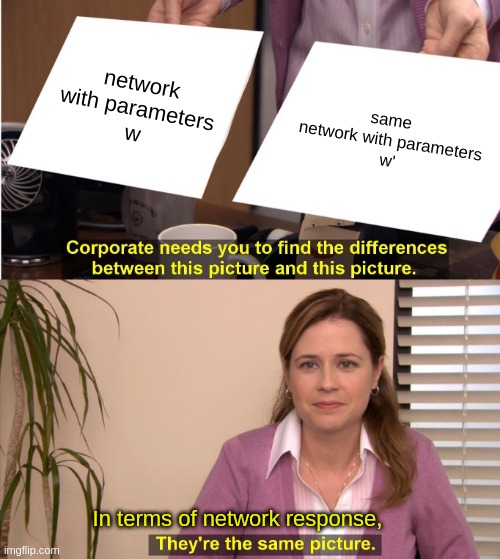
\includegraphics[width=0.3\textwidth]{img/meme_symmetry}
\end{center}
}
  
\end{frame}

\subsection{Permutation of indices within consecutive layers}

\begin{frame}\frametitle{\subsecname}

\mode<presentation>{
\begin{equation*}
y(\vec x; \vec w) = y(\vec x; \vec w')
\end{equation*}
}

We can ensure the same model response and training error $E^{T}$ if:


\begin{equation}
{w'\,}^{v\,v-1}_{ij} = w^{v\,v-1}_{\Pi(i)j}
\end{equation}

for some permutation $\pi$ \underline{and}

\begin{equation}
{w'\,}^{v+1\,v}_{ki} = w^{v+1\,v}_{k\pi(i)}
\end{equation}

then neuron $(v, i)$ behaves identically to neuron $(v, \pi(i))${}

$N_{v}!$ is the total number of possible permutations per hidden layer $v$.

  
\end{frame}

\subsection{Sign-reversal across layers}

\begin{frame}\frametitle{\subsecname}

\mode<presentation>{
\begin{equation*}
y(\vec x; \vec w) = y(\vec x; \vec w')
\end{equation*}
}

We can ensure the same model response and training error $E^{T}$ if:


\begin{align}
{w'\,}^{v\,v-1}_{ij} =& -w^{v\,v-1}_{ij}\,,\\
{w'\,}^{v+1\,v}_{ki} =& -w^{v+1\,v}_{ki} \; \text{and}\\
f^{v}(h) = f^{v+1}(h) :=& \tanh(h),
\end{align}

since $\tanh$ is an odd function: $\tanh(-h) = -\tanh(h)$.

$2^{N_{v}}$ is the total number of sign-reversal combinations per hidden layer $v$.

Both types of symmetries give us 
a total of $\prod_{v=1}^{L} N_{v}!\, 2^{N_{v}}$ eqivalent solutions\notesonly{ (same response, same $E^{T}$). This is true for global and local minima.
It implies that solutions of MLPs with 2 or more hidden layers are not unique.}

  
\end{frame}

